% Chapter Template
\chapter{4 Tensor Decomposition} % Main chapter title
\label{Chapter4}
\def \path	{Figures/C4}

In this chapter the main mathematical tools for the manipulation of tensors are introduced. 
Following, we will see how to apply these operators to decompose a convolutional layer through two different techniques, effectively exploring the state-of-the-art methods of low-rank approximation presented in Chapter 2.

%--------------------------------------------------------------------
%	SECTION 1
%--------------------------------------------------------------------
\section{Background}}
\label{sec:bg}
%% intro 
[A better introduction to tensors is needed. !!]\\
A tensor is a geometric object that generalizes all the structures usually defined in linear algebra to the \emph{n}-dimensional space. As such, they can be defined as \emph{n}-dimensional arrays. \\
Given a reference basis of vectors - i.e. a set of linearly independent vectors with which we can represent every other vector in the correspondent vector space - (cite needed) a tensor can be represented as a multidimensional array of numeric values. We define \emph{rank} (or order) of a tensor the dimensionality of the array needed to represent it with respect to this basis, or the number of indices needed to label a component of that array. Thus, an \emph{k-th} order tensor in an \emph{n}-dimensional space is a mathematical object that has \emph{n} indices and $n^k$ components; each index ranges over the number of dimensions of the space. 

A third-order tensor is showed in \ref{fig:tensor}. 

\subsection{Tensor rank} 
\label{subsec:tensor-rank}
Intuitevely, a scalar would be a tensor of \emph{order 0}; a vector of \emph{order 1}; a matric of \emph{order 2} and so on. 

The intuitive definition can also be used using "\emph{rank}" instead of order, but that may be somewhat misleading since there's a subtle difference. To avoid confusion, the following definitions are introduced: 
\begin{itemize}
  \item a tensor of \emph{rank}-1 or a decomposable tensor \parencit{tensor-hackbush2009} is a tensor that can be written as a product of a product of tensors of the form: 
  \begin{equation}
  \label{eq:rank1-tens}
    T = a \circ b \circ \ldots \circ d  
  \end{equation}   
  
  \item The \emph{rank} of a tensor $T$ is the minimum number of rank-1 tensor that sum to $T$.

\end{itemize}

The product used in \ref{eq:rank1-tens} is an outer product for vectors and will be defined in detail in the coming section. 

Tensors are extensively used in many applications \parencite{WTensor} to modelize multi-dimensional data. In the CNN scenario, a CONV layer with $\mathcal{W}$ weights is defined through a tensor of size: 
\begin{equation}
\label{eq:conv-tensor}
  dim(\mathcal{W})  = [T \times S \times D \times D]
\end{equation}

where, 
\begin{itemize}
 \item $T$ is the number of output filters
 \item $D$ is the size of the kernel of the convolution 
 \item $S$ is the number of input filters 
\end{itemize}

In pure mathematical terms, there exist a lot of different methods to decompose a tensor. In section \ref{sec:tensor-math} the formal tools to wield tensors are given and in section \ref{sec:cpd-application}  the application of these methods to convolutional layers are presented. 

\subsection{Singular value decomposition}
%% SVD Applied on Fully Connected layer 
In order to understand better how a tensor decomposition work and its properties, it is necessary to introduce the \emph{singular value decomposition} (SVD) for matrices. 

Let $M$ be a matrix $\in \mathbf{F}$ of size $m \times n$, the SVD is given by:
\begin{equation}
\label{eq:svd}
   M = U \Sigma V^*
\end{equation}

Where $U$ and $V$ are an $m \times m$ and $n \times n$ unitary matrix respectively. In the case of $\mathbf{F}= \mathbf{R}$, $U$ and $V$ are also orthogonal matrices. $V^∗$ is the conjugate transpose of $V$.  $\Sigma$ is a \emph{diagonal} matrix with non-negative real numbers, which holds the singular values of $M$ in its diagonal. 


A thorough explanation of the above terms is required, so the following definitions must be kept in mind: 
\begin{itemize} 
 \item A \emph{diagonal} matrix is a matrix whose values are all zero except for those on the diagonal. A special case of diagonal matrix is an \emph{identity} matrix, where all these diagonal elements are equal to 1. 
 
 \item Given a matrix $M$, the \emph{transpose} is an operator that flips $M$ over its diagonal producing another matrix $M^T$ as a result, whose column and rows indices are therefore also switched. Hence, the rows of $M$ becomes the columns of $M^T$ and viceversa. 
 
 \item Given a matrix $M \in \mathbf{C}$, its \emph{complex conjugate}, $\bar{M}$, is the conversion of each element $m_{i,j}$ to its conjugate i.e., the real part are the same while the imaginary part have opposite sign and same magnitude. 
 
 \item A \emph{conjugate transpose} is a matrix $M^*$ who's been obtained by first transposing $M$ and then taking the \emph{complex conjugate} of each entry. Also, the following properties holds: 
 		$$
 		M^* = \bar{(M)}^T = \bar{M*T}
 		$$  
 
 \item A quadratic matrix $M$ is said to be \emph{unitary} if $MM^* = M*M = I$, where $I$ is the identity matrix. In the case $M \in \mathbb{R}}$ the matrix is called \emph{orthogonal} and it satisfies the equivalence $MM^T = M^TM = I$. 
 
 \item An \emph{orthogonal} matrix has rows and columns that are unitary or orthogonal between each other, respectively. 
 
 \item A non-negative real number $\sigma$ is a singular value for $M$ of a space $F^{m \times n}$ if and only if there exist unit-length vectors  $u \in \mathbf{F}^m, \, v \in \mathbf{F}^n$ such that $Mv=\sigmau$ and $M^*u=\sigmav$. The vectors $u$ and $v$ are called left-singular and right-singular vectors for $\sigma$ respectively. 

\end{itemize}

Recalling the SVD definition \ref{eq:svd}, the $\m \times n$ rectangular matrix $\Sigma$ holds the  \emph{singular values} (the square roots of the non-zero \emph{eigen-values})  $\sigma_i \: i=1, \ldots, k$ of $M$ on its diagonal. The first $k = min(m,n)$ columns of $U$ and $V$ are, respectively, left-singular vectors and right-singular vectors for the corresponding singular values. Consequently, the SVD theorem implies that: 
\begin{itemize}
	\item An $m \times n$ matrix $M$ has at most $k$ distinct singular values; 
    \item It is always possible to find a unitary basis $U$ for $\mathbf{F}^m$ with a subset of basis vectors spanning the left-singular vectors of each singular value of $M$; 
    
    \item It is always possible to find a unitary basis $V$ for $\mathbf{F}^n$ with a subset of basis vectors spanning the right-singular vectors of each singular value of $M$.
\end{itemize} 


\subsection{SVD Applications}
The SVD factorization is useful in  many fields of research. It can be used to solve the \emph{linear least-squares} and the \emph{total least-squares} problems; it is widely used in statistics where it is related to \emph{principal component analysis} (PCA); it's successfully used in signal processing and pattern recognition. SVD is also fundamental in \emph{recommender systems} to predict people's item ratings \parencite{recsys1} \parencite{recsys2}; for instance, Netflix has launched a global competition to find the best implementation of SVD for clusters to improve its collaborative filtering technique \parencite{recsys3-netflix}. The main area of interest of SVD for convolutional neural networks is that of \emph{low-rank matrix approximation} and image processing. 

In fact, SVD can be thought of as decomposing a matrix into a \emph{weighted, ordered} sum of separable matrices. Separable here means exactly the same concept introduced for tensors in section \ref{subsec:tensor-rank} i.e., a matrix $A$ can be written as an outer product of two vectors $A = u \circ v$. More precisely, the matrix can be factorized as: 
\begin{equation}
  M = \sum_i A_i = \sum_i \sigma_i U_i \circ V_{i}^{T}  
\end{equation} 

this turns out to be enable a fast convolution computation: 

\begin{equation}
	F = \sum_{i}^{R} \sigma_i(I * U_i)*V_i  
\end{equation}

where I is the input image, $F$ is the resultant feature map and $U_i$ and $V_i$ are i-th column of $U$ and $V$ respectively. 

Note that $\sigma_i$ are the R largest singular values (the other singular values are replaced by zero). Since the number of non-zero $\sigma_i$ correspond exactly to the rank of a matrix, the approximated matrix is thus of rank R. \\
For this purpose, given a matrix $M$, the best method to find a truncated matrix $\tilde{M}$ of rank $R$ that approximates $M$, is to find the solution that minimizes the \emph{frobenius norm} of their difference:
\begin{equation}
\left \| M - \hat{M} \right \|, \quad with \ \hat{M} = \sum_i U_i \circ V_i
\end{equation}

The Eckart-Young theorem \parencite{Weckart} states that the best solution to the problem is given by its SVD decomposition. 


\subsubsection{SVD on Convnets}


$$ (U_{n \times t}\Sigma_{t \times t}V^T_{m \times t})x + b $$ = $$ U_{n \times t} ( \Sigma_{t \times t}V^T_{m \times t} x ) + b $$



%--------------------------------------------------------------------
%	SECTION 2
%--------------------------------------------------------------------
\section{Tensor mathematical tools}
\label{sec:tensor-math}

\subsection{Basic operations}
In multi-linear algebra it actually does not exist a method that satisfy all SVD properties for \emph{m-way arrays}, i.e. tensors. However, by taking a closer look at SVD we can formulate two main requirements that a tensor decomposition algorithm should satisfy to be a feasible alternative to SVD in a tensor-world: 
{\begin{enumerate}
	\item a Rank-\mathit{R} decomposition
	\item the orthonormal row/column matrices.
\end{enumerate}}

SVD computes both of them simultaneously. Regarding tensors, these properties can be captured separately by two different family of decompositions.

The first property is extended to the multi-linear world by a class of decompositions that fall under the name of \textit{CP decomposition} (named after the two most popular variants, CANDECOMP and PARAFAC). The latter is provided by the Tucker methods (and many other names). For each axes of a tensor, these methods compute the associated orthonormal space. Therefore, Tucker methods are also used in multilinear principal component analysis (PCA). \\
Historically, much of the interest in higher-order SVDs was driven by the need to analize empirical data, expecially in psychometrics, chemometrics and neuroscience (CIT NEEDED). As such, these techniques have been rediscovered many times with different names leading to a confused literature. Thus, these methods are often presented in a more practical goal-driven way, rather than through rigourous abstract general theorems, which are in fact rare.\\

Before diving into tensor decomposition algorithms, we need to introduce some fundamental tensor operations: 

\begin{itemize}
    \item  \textbf{Tensor times matrix: \textit{k}-mode product:} 
            The $k$-mode product of a tensor X $\in \mathbb{R}^{I_{1} \times I_{2} \times \ldots \times I_{N}}$ with a matrix $M \in \mathbb{R}^{J \times I_{k}}$ is written as: 
           \begin{equation}
                \textbf{Y} = \textbf{X} \times_{k} M
           \end{equation}
            The resulting tensor $Y$ is of size $I_{1} \times \ldots \times I_{k-1} \times J \times I_{k+1} \times \ldots \times I_{N}$, and contains the elements:

            $$ 
             y_{i_{1}  \cdots  i_{k-1}  j  i_{k+1}  \cdots  i_{N}} =   \sum_{i_{k} = 1}^{I_{k}} x_{i_{1}  i_{2}  \cdots  i_{N}} a_{ji_{k}}.
            $$
             
             It can be hard to visualize this operation at first, but effectively it boils down to 
             multiply each mode-\textit{k} fiber of X by the matrix M. Looking at \ref{fig:unfolding}, we can also represent the same operation with 
             $ \textbf{Y}_{(i)} = \textbf{X}_{(i)} \cdot M$, being $X_{(i)}$ the mode-i unfolding of the tensor X. \newline
             
             To simplify things, let \textbf{X} be a 3-mode tensor $\in F^{I \times J \times K}$ and $M$ a matrix $\in F^{N \times J}$, the k-mode product on axis 1 of X and M is:
            
            \begin{equation}
                        \textbf{Y} = \textbf{X} \times_{1} M, Y \in F^{I \times J \times K} 
            \end{equation}
            So each element (\textit{n, j, k}) of Y is obtained by: 
            \begin{equation}
                y_{n,j,k} = \sum_{i} x_{i,j,k}  \cdot  b_{n,j}  
            \end{equation}
            
            A visual example is depicted in \ref{k-mode}.
            
                        
            Few interesting properties of the k-mode product are: \\
            \begin{itemize}
                \item  $\tensor{X} \times_{m} A \times_{n} B = \tensor{S} \times_{n} B \times_{m} A$ if $n \neq m$ \\
                
                \item  $X \times_{n} A \times_{n} B = \tensor{X} \times_{n} (BA)$ $\neq \tensor{X} \times_{n} B \times_{n} A$.
            \end{itemize}

    
    \item \textbf{Tensor times vector}: 
       Given the same matrix X, the tensor-vector multiplication on the \textit{i}-axis is defined as:
       \begin{equation}
           \textbf{Y} = \textbf{X} \times_1 v, \textbf{Y} \in \mathbb{}
       \end{equation}

        with each element $y_{j,k}$: 
        \begin{equation}
            y_{j,k} = \sum x_{i,j,k} \cdot a_i
       \end{equation}
       
       An example is illustrated in \ref{fig:tensor-to-vec}.
        
    \item \textbf{Matrix Kronecker product}: 
       A Kronecker product of two matrices $A \in \mathbf{R}^{M \times N}$ and $B \in \mathbf{R}^{P \times Q}$
       is defined as: 
        \begin{equation} 
        A\otimes B = \begin{bmatrix} a_{11} B & \cdots & a_{1n}B \\ \vdots & \ddots & \vdots \\ a_{m1} B & \cdots & a_{mn} B \end{bmatrix}
        \end{equation}
        
        and more explicitly: %% KRONCKER MATRICIONE!!! %% 
        $$
        MATRICIONE
        $$
        
    
    \item \textbf{Outer product}: If we take the \emph{Kronecker product for matrices} definition and apply it to vectors, we obtain the outer product: \\
        
        \begin{align}
            \mathbf{a} \circ \mathbf{b} = \mathbf{a} \mathbf{b}^\mathrm{T}
            = \begin{bmatrix}a_1 \\ a_2 \\ a_3 \\ a_4\end{bmatrix}
            \begin{bmatrix}b_1 & b_2 & b_3\end{bmatrix}
            = \begin{bmatrix}a_1b_1 & a_1b_2 & a_1b_3 \\ a_2b_1 & a_2b_2 & a_2b_3 \\ a_3b_1 & a_3b_2 & a_3b_3 \\ a_4b_1 & a_4b_2 & a_4b_3\end{bmatrix}.
        \end{align}

        Let $a \in \mathbf{R}^I$, $b \in \mathbf{R}^J$  $c \in \mathbf{R}^K$ be three vectors. Computing the outer 
        product ($a  \circ  b$) of two of them will result in a matrix, as showed above. Proceeding in this way is easy to show that an outer product of 3-vectors will result in a 3-dimensional tensor, as illustrated in \ref{fig:outer-product}.
        
        This comes in handy the other way around: a rank-1 tensor can be decomposed into 3 vectors. As we will see in the following sections, this operation is fundamental for tensor decomposition.
        
        Another interesting way to look at it is that the outer product operation “◦” is a way of combining a tensor of $d1$-order and a tensor of $d2$-order to obtain a tensor of order-$(d1+d2)$.

    \item \textbf{Matrix Khatri-Rao product}: given two matrices $A \in \mathbf{R}^{M \times N}$ and $B \in            \mathbf{R}^{P \times R}$ is defined as: 
        \begin{equation}
            A \odot B = [a_1 \otimes b_1, a_2 \otimes b_2, \ldots, a_N \otimes b_R] \in \mathbf{R}^{MN \times R}
        \end{equation}
        
        Note that the Kronecker matrix operation returns the same number of elements of the Khatri-Rao product, but while the former produce a matrix, the latter is shaped into a vector.   

\end{itemize}


\subsection{Tucker Decomposition}


\subsubsection{HO-SVD}
As the \emph{Higher-order singular value decomposition} was studied in many scientific fields, it is historically referred in different ways:  multilinear singular value decomposition, m-mode SVD, or cube SVD, and it is often incorrectly identified with a Tucker decomposition. 

HOSVD is actually a specific orthogonal version of the Tucker decomposition. To put it in other words, it is a specialized algorithm to compute the Tucker decomposition. HOSVD involves solving each \emph{k}-mode matricized form of the specific tensor \parencite{WTucker}, relying on the following equivalence: \\

	\begin{eqnarray}
	\centering
	Y &=& X \times_{1} A^{(1)} \times_{2} A^{(2)} \times_{3} \ldots \times_{N} A^{(N)} \nonumber\\
	\Leftrightarrow \quad Y_{(k)} &=& A^{(k)} X_{(k)} \left(A^{(N)} \otimes \cdots \otimes A^{(k+1)}   \otimes A^{(k-1)} \otimes \cdots A^{(1)} \right)^T. \nonumber
	\end{eqnarray}

The algorithm steps follow: 
\begin{eqnarray}
&\,&\mathrm{for}\, k = 1, 2, ..., N \,\mathrm{do} \nonumber\\
&\,&\quad A^{(k)} \leftarrow \,\mathrm{left\,orthogonal\,matrix\,of\,SVD\,of}\,X_{(k)} \nonumber\\
&\,&\mathrm{end\,for} \nonumber\\
&\,&G \leftarrow X \times_{1} (A^{(1)})^T \times_{2} (A^{(2)})^T \times_{3} \cdots \times_{N} (A^{(N)})^T  \nonumber
\end{eqnarray} 

This approach may be regarded as one generalization of the matrix SVD, because:
\begin{itemize}
	\item each matrix $\mathit{A}^k$ is an ortoghonal matrix 
	\item Two subtensors of the core tensor $\mathbf{G}$ are orthogonal, i.e. $\left \langle \mathbf{G}_p , \mathbf{G}_q \right \rangle \quad if \quad p \neq q$
	\item the subtensors in the core tensor $\mathbf{G}}$ are ordered according to their Frobenius norm, i.e. $\left \| \mathbf{G}_1 \right \|  \geq  \left \| \mathbf{G}_2 \right \| \geq \ldots  \geq \left \| \mathbf{G}_n \right \|_{\: for \: n=1,\ldots,N} $
\end{itemize}
	
The tensor $\mathbf{G}$ is said to be \emph{"ordered"} and \emph{"all-ortoghonal"}. For further explanation see \parencite{multilinear}. 






\begin{equation}
    \mathrm{X} = \mathbf{G} \times_{1} A^{(1)} \times_{2} A^{(2)} \times_{3} \ldots \times_{N} A^{(N)}
\end{equation}

\subsection{Canonical Polyadic Decomposition}
\begin{comment}
$\tensor{A} \otimes \tensor{B}$ denote the outer product between an $N\th$-order tensor $\tensor{A}$ and an $M\th$-order tensor $\tensor{B}$, then $\tensor{A} \otimes \tensor{B}$ is the $(N+M)\th$-order tensor defined by $(\tensor{A} \otimes \tensor{B})_{i_1\cdots i_N\,j_1\cdots j_M} = a_{i_1\cdots i_N} \cdot b_{j_1\cdots j_M}$. 
\end{comment}
%% rivedere %% 
The Polyadic Decomposition (PD) \parencite{tensor2009kolda} approximates a tensor with a sum of $R$ rank-one tensors. If the number of rank-one terms $R$ is minimal, then $R$ is called the rank of the tensor and the decomposition is called minimal or \emph{canonical} (CPD). \\
For any other arbitrary \mathit{rank-r}, the decomposition is often referred to as CANDECOMP/PARAFAC (CP). As we will discover later, selecting the perfect rank is an \emph{NP-Hard} problem. Hence, from now on we will refer to this decomposition as CP. \newline 

Recall the outer product between vectors introduced in section \ref{sec:tensor-math}.
Let $\vec{a}$, $\vec{b}$ and $\vec{c}$ be nonzero vectors in $\mathbf{R}^{n}$, then $\vec{a} \circ \vec{b} \equiv \vec{a}\cdot \vec{b}^{\T}$ is a rank-one matrix and
$\vec{a} \circ \vec{b} \circ \vec{c}$ is defined to be a rank-one tensor. Let $\ten{T}$ be a tensor of dimensions $I_1 \times I_2 \times \cdots
\times I_N$, and let $\mat{U}^{(n)}$ be matrices of size $I_n \times R$ and $\vec{u}_r^{(n)}$ the $r$\th column of $\mat{U}^{(n)}$,
then:

\begin{equation}
    \ten{T} \approx \sum_{r=1}^{R} \vec{u}^{(1)}_r \circ \vec{u}^{(1)}_r \circ
   \cdots \circ \vec{u}^{(N)}_r.
\end{equation} 

A visual representation of this decomposition in the third-order case is shown
in \ref{fig:cpd}

It's interesting to notice that CPD can be regarded as a special case of a Tucker Decomposition in which the core tensor $\mathbf{G}$ is constrained to be a super-identity I, which is an extension of the identity matrix and has all one's on its superdiagonal and all zero's off the superdiagonal. 




%--------------------------------------------------------------------
%	SECTION 3
%--------------------------------------------------------------------
\section{Application of tensor decompositon on CNN}
\label{sec:cpd-application}
\subsection{Convolutional layer as 4-mode tensors}

\subsection{CPD}

\begin{equation}
$$ \sum_{r=1}^R K^x_r(i)K^y_r(j)K^s_r(s)K^t_r(t) $$.	
\end{equation}


%%%% forward pass con CPD %%% 
\begin{center}
\begin{align*}
	V(x, y, t) = \sum_i \sum_j \sum_s K(x-i, y-j, s, t)X(i, j, s) \\
		= \sum_r \sum_i \sum_j \sum_s K^x_r(x-i)K^y_r(y-i)K^s_r(s)K^t_r(t)X(i, j, s)\\
			= \sum_r K^t_r(t) \sum_i \sum_j K^x_r(x-i)K^y_r(y-i) \sum_s K^s_r(s) X(i, j, s) \tag{4}
\end{align*}
\end{center}


\subsection{Tucker}
%% forward pass con Tucker 
The Tucker Decomposition, also known as the Higher Order SVD  \emph{HOSVD} is a generalization of SVD for tensors: 

$$ K(i, j, s, t) = \sum_{r_1=1}^{R_1}\sum_{r_2=1}^{R_2}\sum_{r_3=1}^{R_3}\sum_{r_4=1}^{R_4}G_{r_1, r_2, r_3, r_4} * K^x_{r1}(i)K^y_{r2}(j)K^s_{r3}(s)K^t_{r4}(t) $$

The Tucker Decomposition has a property that's useful for our purposes: it doesn't have to be applied along all modes (axis) of the tensors. We have seen how CPD decomposes the kernel also spatial-wise; this acts
pretty aggressively on the number of parameters and since the convolutional kernels are small in most of the recent implementations ($3 \times 3$ or $5 \times 5$) it arguably doesn't save a lot of computation. Hence, we can skip
this decomposition with Tucker, going for what is known as a Tucker-2 Decomposition: 

\begin{equation}
\label{eq:tucker-def}
	K(i, j, s, t) = \sum_{r_3=1}^{R_3}\sum_{r_4=1}^{R_4} \textbf{G} {i,j,r_3, r_4}(j)K^s_{r3}(s)K^t_{r4}(t) 
\end{equation} 

Using equation \ref{eq:tucker-def} and plugging into the formula for the convolutional forward pass, we obtain the new equation for the Tucker convolutional forward pass: 

\begin{equation}
V(x, y, t) = \sum_i \sum_j \sum_sK(x-i, y-j, s, t)X(i, j, s) 

\end{equation}

\begin{equation}
V(x, y, t) = \sum_i \sum_j \sum_s\sum_{r_3=1}^{R_3}\sum_{r_4=1}^{R_4}\mathbf{G}(x-i)(y-j) r_3 r_4}K^s_{r3}(s)K^t_{r4}(t)X(i, j, s) 
\end{equation}

\begin{equation}
V(x, y, t) = \sum_i \sum_j \sum_{r_4=1}^{R_4}\sum_{r_3=1}^{R_3}K^t_{r4}(t)\mathbf{G}(x-i)(y-j) r_3 r_4} \sum_s\ K^s_{r3}(s)X(i, j, s) 
\end{equation}

%%inserire codice per dataset MNIST %% 
%--------------------------------------------------------------------
%	SECTION 4
%--------------------------------------------------------------------
\section{MNIST: addestramento}


%--------------------------------------------------------------------
%	SECTION 5
%--------------------------------------------------------------------
\section{CIFAR: preprocessing}




%--------------------------------------------------------------------
%	SECTION 6
%--------------------------------------------------------------------
\section{CIFAR: addestramento}




%%%%%%%%%%%%%%%%%%%%%%%%%%%%%%%%%%%%%%%%%%%%%%%%%%
%%%%%%%%%%%%%%%%%%%%%%%%%%%%%%%%%%%%%%%%%%%%%%%%%%

%% Approximation with CPD 







\begin{lstlisting}[language={[5.2]Lua}]
----- preprocess/normalize train/test sets -----
print '<trainer> preprocessing data (color space + normalization)'

-- preprocess trainSet
normalization = nn.SpatialContrastiveNormalization(1, image.gaussian1D(7))
for i = 1,trainData:size() do
   --rgb -> yuv
   local rgb = trainData.data[i]
   local yuv = image.rgb2yuv(rgb)
   
   -- normalize Y locally:
   yuv[1] = normalization(yuv[{{1}}])
   trainData.data[i] = yuv
end
-- normalize U globally:
mean_u = trainData.data[{ {},2,{},{} }]:mean()
std_u = trainData.data[{ {},2,{},{} }]:std()
trainData.data[{ {},2,{},{} }]:add(-mean_u)
trainData.data[{ {},2,{},{} }]:div(-std_u)

-- normalize V globally:
mean_v = trainData.data[{ {},3,{},{} }]:mean()
std_v = trainData.data[{ {},3,{},{} }]:std()
trainData.data[{ {},3,{},{} }]:add(-mean_v)
trainData.data[{ {},3,{},{} }]:div(-std_v)

--same applies to test set...
\end{lstlisting}



\begin{figure}[h!]
 \centering
 \includegraphics[width=1.0\textwidth]{\path/k-mode.png} 
  \caption{Example of k-mode multiplication on 3-dimensional tensor.}
 \label{fig:k-mode}
\end{figure}

\bigskip

\begin{figure}
\centering
\begin{subfigure}{.5\textwidth}
  \centering
 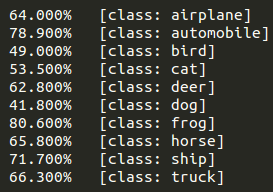
\includegraphics[width=1\textwidth]{\path/cifar-tanh.png} 
  \caption{Acc.= \textasciitilde 65\% f. di attivazione = TanH}
 \label{fig:training}
\end{subfigure}%
\begin{subfigure}{.5\textwidth}
  \centering
 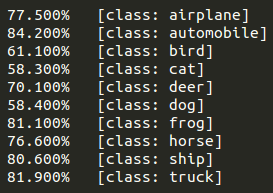
\includegraphics[width=1\textwidth]{\path/cifar-relu.png} 
  \caption{Acc.= \textasciitilde 73\% f. di attivazione = ReLU}
 \label{fig:validation}
\end{subfigure}
\caption{Percentuali di accuracy a seconda della funzione d'attivazione. La ReLU produce indubbiamente risultati migliori.}
\label{fig:relu}
\end{figure}
\\
%%%%% NEW PAGE FOR THE NEW FIGURES %%%% 
\newpage
\pagebreak
\medskip
\newpage

\begin{figure}[h!]
 \centering
 \includegraphics[width=1.0\textwidth]{\path/tensor-mode.jpg} 
 \caption{Fibers and slices of a tensor: fibers is an equivalent term for a tensor mode.}
 \label{fig:tensor-fibers}
\end{figure}

\begin{figure}[h!]
 \centering
 \includegraphics[width=1.0\textwidth]{\path/tucker-pass.jpg} 
 \caption{Tucker-2  Decompositions  for  speeding-up  a generalized convolution. Each box corresponds to a 3-way tensor $X, Z, Z^' and Y$ in equation (\ref{eq:tucker1}-\ref{eq:tucker3}). Arrows represent linear mappings 
and illustrate each scalar value on the right is computed. Red tube, green cube and blue tube correspond to 
1x1, dxd and 1x1 convolution respectively.}
 \label{fig:tucker-pass}
\end{figure}


\begin{figure}[h!]
 \centering
 \includegraphics[width=1.0\textwidth]{\path/CPD.jpg} 
 \caption{Tensor Decompositions for speeding up a generalized convolution. Each box correspond to a feature map stack within a CNN, (frontal sides are spatial dimensions). Arrows show linear mappings and demonstrate how scalar values on the right are computed. Initial full convolution (A) computes each element of the target tensor as a linear combination of the elements of a 3D subtensor that spans a spatial d × d window over all input maps. 
Jaderberg et al. (B) approximate the initial convolution as a composition of two linear mappings in which the intermediate mpa stack has R  maps, being R the rank of the decomposition. Each of the two-components 
computes each target value with a convolution based on a spatial window of size dx1 or 1xd in all input maps. Finally, CP-decomposition (C) by Lebedev et al. approximates the convolution as a composition of four smaller convolutions: the first and the last components compute a standard 1x1 convolution that spans all input maps while the middle ones compute a 1D grouped convolution \textbf{only on one} input map.}
 \label{fig:cpd-pass}
\end{figure}


